In this section, we evaluate the performance of our simulation tool.
We show that the inclusion of multiple synchronization protocols does not decrease our performance to the point where it is unusable.
To this end, we compare to adevs, one of the most efficient simulation kernels at this time~\cite{DEVSSurvey}.
A comparison is made for both the CPU and memory usage of both sequential simulation and parallel simulation.

We start of with a comparison of sequential simulation, to show how adevs and dxex relate in this simple case.
We not only show that our approach does not influence performance negatively, but also that our main simulation algorithm, similar to the one of PythonPDEVS, is significantly faster than the one found in adevs.
Similar differences, compared to adevs, can also be seen in the parallel simulation benchmarks.
In the parallel simulation benchmarks, the benefit of our different synchronization protocols is also indicated.

For all benchmarks, results were all well within 1\% deviation of the average, such that only the average is used in the remainder of this section.
The same compilation flags were used for both adevs and dxex benchmarks (``\texttt{-O3}'').
To guarantee comparable results, no IO was performed during the benchmarking phase.
Simulation traces were used to verify that both adevs and dxex models have exactly the same behaviour.
All benchmarks were performed using Linux, but our simulation tool works equally well on Windows and Mac.

\subsection{Benchmarks}
We use a selection of benchmarks, based on those found in the literature.
Three different types of benchmark are defined, each for a different purpose:
\begin{enumerate}
    \item \textit{Queue} model, based on the HI model of DEVStone~\cite{DEVStone}, creates a chain of atomic models, which are hierarchically nested in each other.
          A single generator will push events into the queue, which get processed by the processors after a fixed or random delay.
          It takes two parameters: width and depth, which determine the widht and depth of the hierarchy.
          This benchmark shows how the complexity of the simulation kernel behaves with an increasing amount of atomic models, and an increasingly deep hierarchy.
          If the processing delay is fixed for all processors, further insight is provided in the collision handling performance of the simulation kernel.
          An example for width 2 and depth 3 is shown in Figure~\ref{fig:queue_model}.

    \item \textit{PHOLD} model, presented by~\cite{PHOLD}.
          It creates a set of $n$ atomic models, and each model has exactly $n-1$ output ports: one for every other atomic model.
          Couplings are made such that each atomic model is directly connected to each other atomic model, such that every atomic model can directly send an event to every other atomic model.
          After a random delay, atomic models will send out an event to a randomly selected output port.
          Output port selection happens in two phases: first it is decided whether the event should be sent to an atomic model inside or outside of this coupled model.
          Afterwards, a uniform selection is made between the possible ports.
          It takes one parameter: the percentage of remote events, which influences the fraction of messages routed to other coupled models.
          This benchmark shows how the simulation kernel behaves in the presence of many local or remote events.
          An example for four models, split over two nodes, is shown in Figure~\ref{fig:PHOLD_model}.

    \item \textit{HighInterconnect} model, a merge of the HI model of DEVStone~\cite{DEVStone} and PHOLD~\cite{PHOLD}.
          It creates a structure similar to the one from PHOLD, but instead of $n-1$ output ports, every atomic model has only a single output port.
          All models are still connected to each other, but through the use of broadcasting: every model will receive a generated event.
          It takes one parameter: the number of models.
          This benchmark investigates the complexity of the routing algorithm.
          An example for four models is shown in Figure~\ref{fig:interconnect_model}.
\end{enumerate}

We opted to deviate from the DEVStone benchmark, as DEVStone tends towards unrealistic models since all internal and external transitions occur simultaneously.
In our benchmark models, there is always the option for simultaneous transition functions (\textit{fixed time advance}), or scattered transition functions (\textit{random time advance}).
Furthermore, they defined the use of an artificial load function, which easily skews the result, making the actual simulation algorithm barely comparable.

\begin{figure}
    \center
    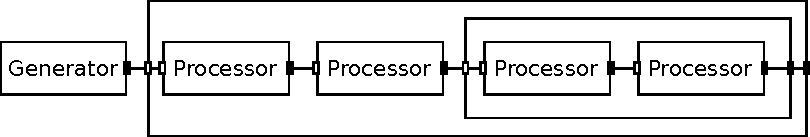
\includegraphics[width=\columnwidth]{fig/queue_model.pdf}
    \caption{Queue model for depth 3 and width 2.}
    \label{fig:queue_model}
\end{figure}

\begin{figure}
    \center
    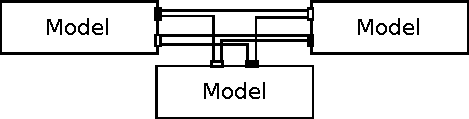
\includegraphics[width=\columnwidth]{fig/interconnect_model.pdf}
    \caption{HighInterconnect model for four models.}
    \label{fig:interconnect_model}
\end{figure}

\begin{figure}
    \center
    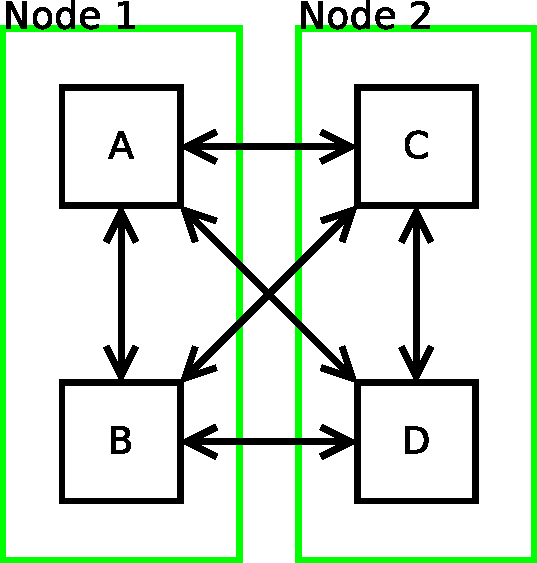
\includegraphics[width=0.5\columnwidth]{fig/phold_model.pdf}
    \caption{PHOLD model for four models, split over two nodes. In parallel simulation, each coupled model is simulated at a different node.}
    \label{fig:PHOLD_model}
\end{figure}

\subsection{Sequential Simulation Execution Time}
Despite our core contribution being mainly in the parallel simulation, we still value a comprehensive comparison of sequential simulation results.
First, and foremost, as parallel simulation results are tightly linked to the sequential simulation results: parallel simulation merely adds a synchronization layer over different, essentially sequential, simulation kernels.
Second, since parallel simulation results are validated through the use of adevs.
To provide a more comprehensive comparison to adevs in the parallel simulation benchmarks, sequential simulation results need to be compared.
Only the Queue and HighInterconnect models are relevant for sequential simulation.

\subsubsection{Queue}
In the Queue model, we increase both the width and depth simultaneously, causing a quadratic growth in the number of atomic models.
As can be seen in Figure~\ref{fig:Queue_benchmark}, dxex considerably outperforms adevs.
Through careful analysis of profiling results, we determined that adevs spends much time in handling simulation messages, whereas this is mostly avoided due to the differently designed simulation algorithm of dxex.
Both simulation tools have quadratically increasing execution times, though dxex is much faster thanks to its more efficient simulation control algorithms.

\begin{figure}
	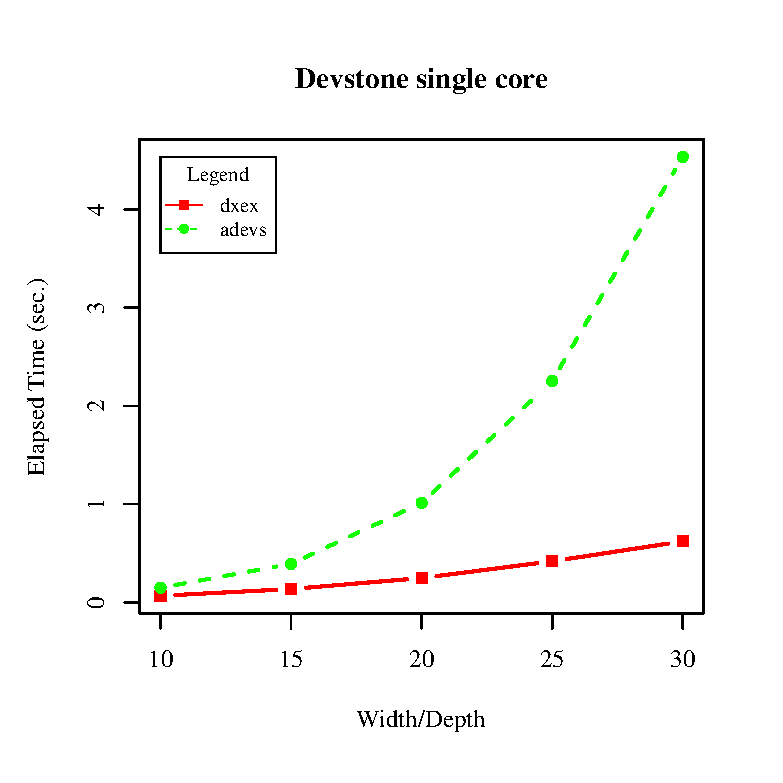
\includegraphics[width=\columnwidth]{fig/fig1.eps}
	\caption{Queue benchmark results for sequential simulation.}
	\label{fig:Queue_benchmark}
\end{figure}

\subsubsection{HighInterconnect}
In the HighInterconnect model, we increase the number of atomic models, thus quadratically increasing the number of couplings.
As can be seen in Figure~\ref{fig:Interconnect_benchmark}, adevs now outperforms dxex by a fair margin.
Analysis showed that this slowdown is caused by the high amount of exchanged events.
Event creation is found to be much slower in dxex than it is in adevs, even despite the use of memory pools in dxex.

%TODO only include sequential results?
\begin{figure}
	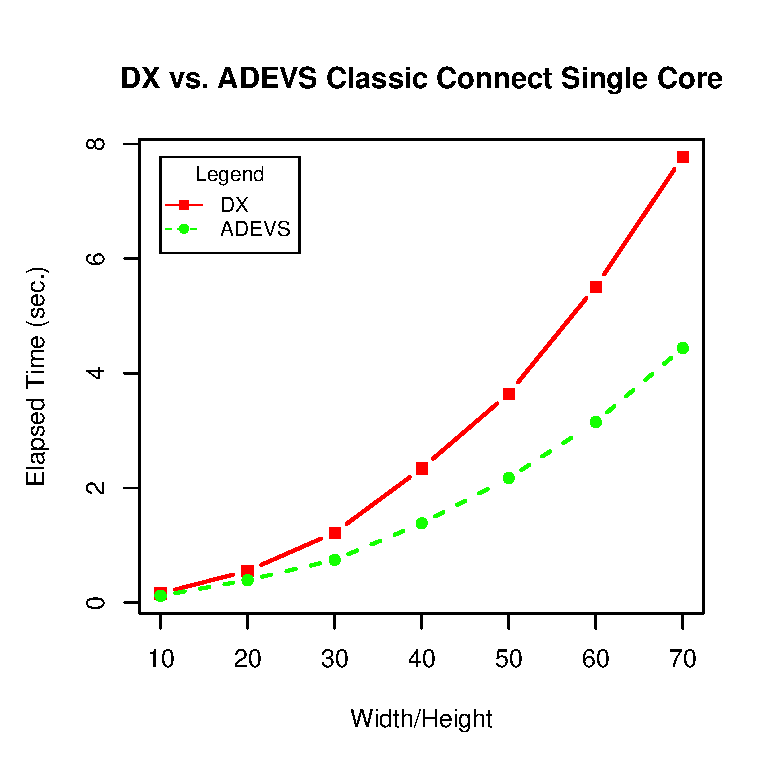
\includegraphics[width=\columnwidth]{fig/fig3.eps}
	\caption{Interconnect benchmark results for sequential simulation.}
	\label{fig:Interconnect_benchmark}
\end{figure}

\subsection{Parallel Simulation Execution Time}
We now perform an analysis of parallel simulation execution times of our previously defined benchmarks.
For dxex, we mention results for both conservative and optimistic synchronization.
Since adevs supports only conservative synchronization, we don't mention optimistic synchronization results there.
All experiments were performed using four simulation nodes, and executed on a quad-core machine.

We highlight two main results:
(1) dxex conservative synchronization is competitive with adevs;
(2) dxex optimistic synchronization is sometimes more efficient than conservative synchronization.
This shows that our contribution, offering both conservative and optimistic synchronization, is indeed beneficial for a general-purpose simulation tools.

\subsubsection{Queue}
In the Queue model, we allocate the chain of models such that each node is responsible for a series of connected models.
This minimizes the number of inter-node messages.
As the model is a queue, however, the last models will only activate much later on in the simulation.
Since these are allocated to seperate nodes, some nodes will remain idle until simulation has progressed sufficiently far.

Similar to the sequential benchmarks, Figure~\ref{fig:queue_benchmark_parallel} shows that dxex again outperforms adevs, using both optimistic and conservative synchronization.
Behaviour is exactly the same as in sequential simulation, but some speedup is achieved.
In this case, conservative synchronization seems to be better than optimistic synchronization, at the cost of providing the lookahead.

\begin{figure}
	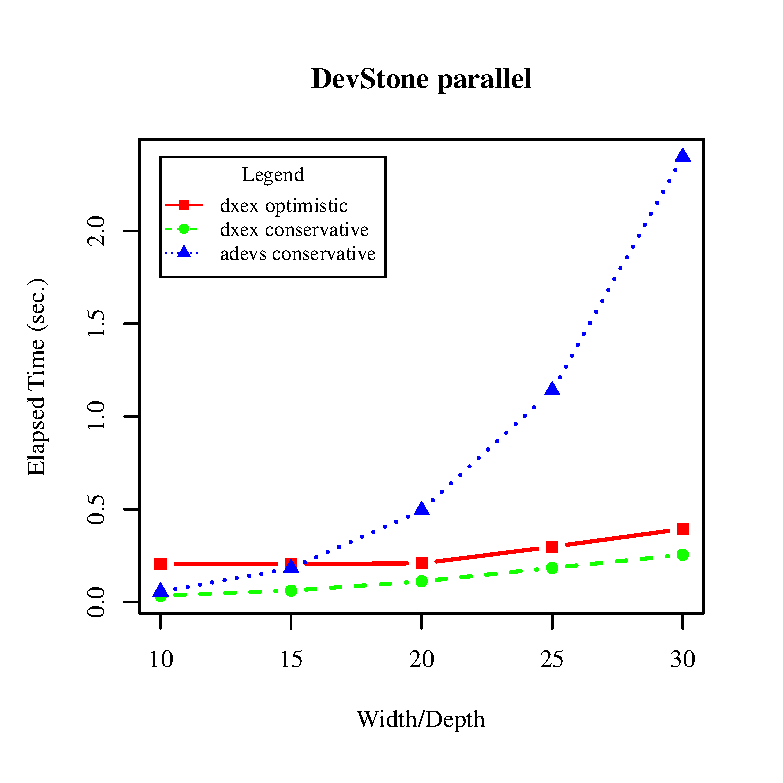
\includegraphics[width=\columnwidth]{fig/fig2.eps}
	\caption{Queue benchmark results for parallel simulation using 4 cores.}
	\label{fig:queue_benchmark_parallel}
\end{figure}

\subsubsection{PHold}
In the Phold model, we first investigate the influence of the fraction of remote events on the speedup.
When remote events are rare, optimistic synchronization will also have rare rollbacks, thus increasing performance.
With more common remote events, however, optimistic synchronization quickly loses its advantage due to the more frequent rollbacks.
Conservative synchronization, on the other hand, is largely unconcerned with the number of remote events: the mere fact that a remote event can happen, causes it to block.
Even though a single synchronization protocol suffices in this case, it shows how different synchronization protocols respond differently to a changing model.
Adevs, on the other hand, is significantly slower during conservative synchronization.
Analysis of profiling results shows that this was caused by exception handling within the adevs simulation kernel.

Secondly, we verify that our contribution fulfills our projected use case: a single model that can be tweaked to favor either conservative or optimistic synchronization.
We slightly modified the Phold benchmark, to include high-priority events.
Contrary to normal events, which offer a sufficiently large lookahead, high-priority events happen almost instantaneous, thus restricting lookahead to a very small value.
Even though the normal events will occur most oftenly, a conservative implementation should always block since these high-priority events can always occur.
An optimistic implementation, however, will simply go forward in simulation time and roll back the few times that these high-priority events happen.
This situation closely mimics the case made in the comparison between both synchronization algorithms by~\cite{FujimotoBook}.

Figure~\ref{fig:phold_priority} shows how simulation performance is influenced by the fraction of high-priority events.
If barely any high-priority events occur, conservative synchronization is penalized due to its excessive blocking, which often turned out to be unnecessary.
Should many high-priority events occur, however, optimistic synchronization is penalized due to its mindless progression of simulation, which frequently needed to be reverted.
These results show that there is no single perfect synchronization algorithm for this model.
Depending on model configuration, either synchronization protocol might be better.
We therefore claim that our contribution is invaluable for high performance simulation: depending on the observed communication behaviour, modellers can use the most appropriate synchronization protocol.

\begin{figure}
    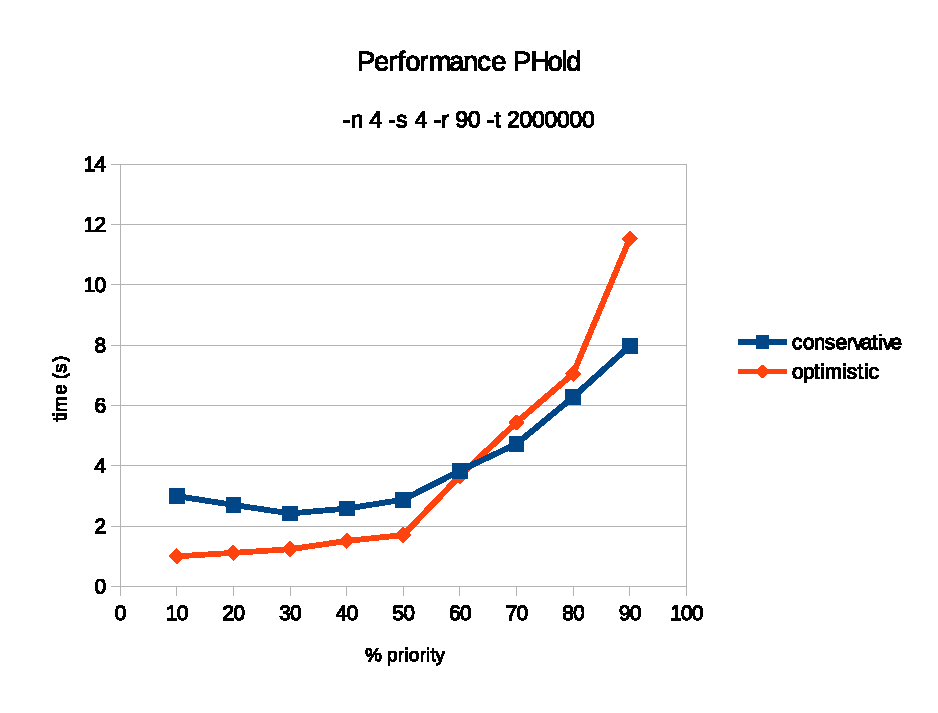
\includegraphics[width=\columnwidth]{fig/phold_voorlopig.eps}
    \caption{Phold benchmark results with high-priority events.}
    \label{fig:phold_priority}
\end{figure}

\subsubsection{Interconnect}
In the Interconnect model, we determine how broadcast communication is supported across multiple nodes.
Results are shown in Figure~\ref{fig:interconnect_benchmark_parallel}
While conservative simulation delivers the expected speedups, dxex is still significantly slower than adevs.
Interestingly, adevs does not achieve any noticable speedup from the use of multiple cores in this situation.
Optimistic synchronization is not shown in this case: due to the high amount of exchanged events, all of which need to be stored in the sending \textit{and} receiving node, it quickly runs out of memory.
Several fixes to this problem have been proposed in the literature~\cite{FujimotoBook}, but none of these is implemented by dxex.

\begin{figure}
    %TODO
    %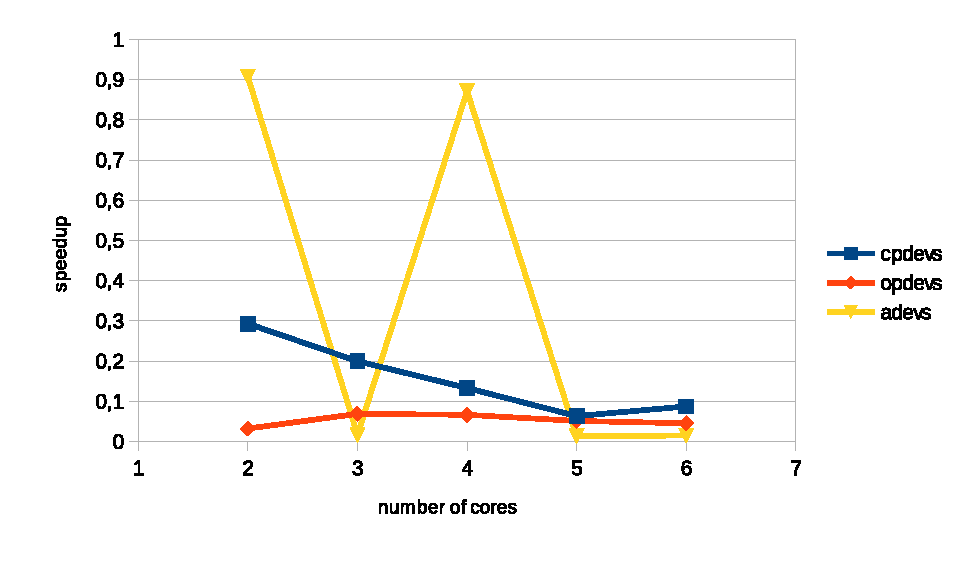
\includegraphics[width=\columnwidth]{fig/interconnect_parallel.eps}
    \caption{Interconnect benchmark results for parallel simulation.}
    \label{fig:interconnect_benchmark_parallel}
\end{figure}

\subsection{Memory Usage}
Apart from simulation execution time, memory usage during simulation is also of great importance.
While execution time only becomes a problem if it takes way too long, coming short only a bit of memory can make simulation infeasible.
We therefore also investigate memory usage of different synchronization protocols.

We do not tackle the problem of states that become too large for a single machine to hold.
This problem can be mitigated by distribution over multiple machines, which neither dxex or adevs support.
Comparison of memory usage should thus only be seen in the context of which models are feasible to be simulated by the tool.

\subsubsection{Remarks}
Both dxex and adevs use tcmalloc as memory allocator.
Additionally, dxex uses memory pools to further reduce the frequency of expensive system calls (\textit{e.g.}, malloc and free).
Tcmalloc only gradually releases memory back to the OS, whereas our pools will not do so at all.
If memory has been allocated once, it is, at least from a performance point of view, better to keep that memory in the pool indefinitely.
Due to our motivation for memory usage analysis, we will only measure peak allocation.
Profiling is done using Valgrind's massif tool~\cite{Nethercote:2007:VFH:1273442.1250746}.

\subsubsection{Results}
Figure~\ref{fig:memory} shows the memory used by each different benchmark.
Results are in megabytes, and show the total memory footprint of the running application (\textit{i.e.}, text, stack, and heap).

Unsurprisingly, optimistic synchronization results show very high memory use due to the saved states.
Note the logarithmic scale that was used for this reason.
Also, results for optimistic synchronization vary heavily depending on thread scheduling by the operating system, as this influences the drift between different nodes.
Comparing similar approaches though, we notice that dxed and adevs have very similar memory use.

Conservative simulation always uses more memory than sequential simulation, as is to be expected.
Additional memory is required for the multiple threads, but also to store all events that are processed simultaneously.

For the Phold benchmark, adevs using conservative synchronization took too long using our profiling tool, and was therefore aborted.
Therefore, no results are shown for adevs.

\begin{figure}
    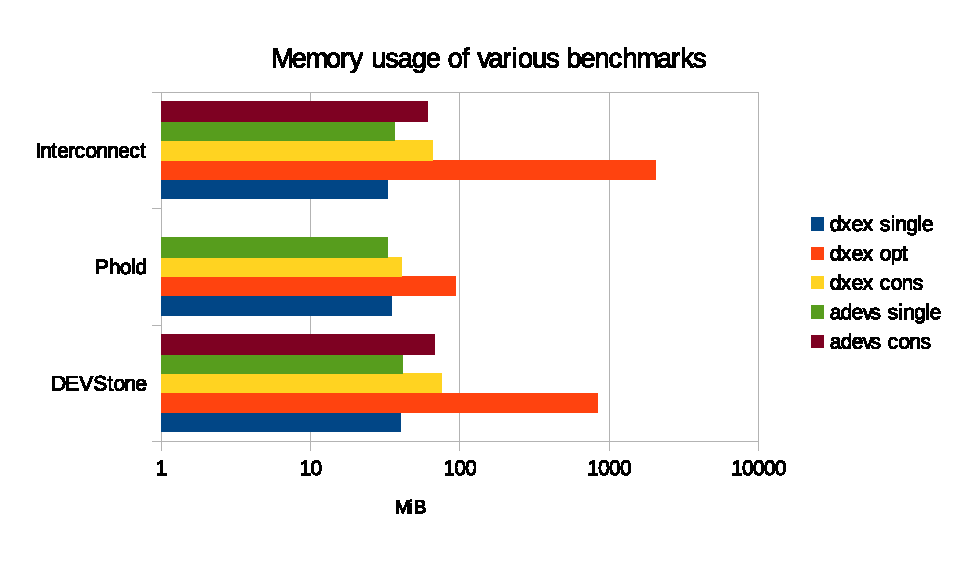
\includegraphics[width=\columnwidth]{fig/memory_voorlopig.eps}
    \caption{Memory usage results.}
    \label{fig:memory}
\end{figure}
